%!TeX root = main.tex
\chapter{Levelt-\!Turrittin-\!Theorem}
Nun zum wichtigsten Satz in dieser Arbeit. Das Levelt-Turrittin-Theorem sagt,
dass sich jeder meromorphe Zusammenhang $\cM$, nach einem möglicherweise
nötigem pull-back, in eine direkte Summe von \glqq elementaren\grqq{}
meromorphen Zusammenhängen zerlegen lässt.\\
Zunächst soll geklärt werden, was die richtigen elementaren meromorphen
Zusammenhänge sind.
\section{Elementare meromorphe Zusammenhänge}
\begin{defn}
Ein \emph{elementarer regulärer meromorpher Zusammenhang} ist ein Zusammenhang
$\cM$, welcher isomorph zu $\cD_{\hat K}/\cD_{\hat K}\cdot
(x\partial_x-\alpha)^p$, mit passendem $\alpha$ und $p$, ist.
\end{defn}
\iffalse
\begin{figure}[htbp]
  \begin{center}
    \begin{tikzpicture}[scale=1,descr/.style={fill=white,inner sep=2.5pt}]
    \def\myPoints{}
    \def\myPath{ -- (3,0)}
    \myPlotFunction[nogrid]{\myPoints}{\myPath}{3}{0}{0}{
      $N((x\partial_x-\alpha)^p)$
    }

    \draw (3,0) -- (3,-.2);
    \node[below] at (3,-.2) {\footnotesize$p$};
    \end{tikzpicture}
  \end{center}
  \caption{Newton-Polygon zu Elementarem regulärem meromorphem Zusammenhang.}
\end{figure}
\fi
\begin{bem}
Es ist leicht zu sehen, dass jeder elementare reguläre meromorphe Zusammenhang
tatsächlich auch regulär ist.
\end{bem}

\begin{lem}
Es existiert eine Basis von $\cM_{\hat K}$ über $\hat K$ mit der Eigenschaft,
dass die Matrix, die $x\partial_x$ beschreibt, nur Einträge in $\Cfx$ hat.
\end{lem}
\begin{comment}
\cite[Lem 5.2.1.]{sabbah_cimpa90}
\end{comment}
\begin{proof}
Wähle einen zyklischen Vektor $m\in\cM_{\hat K}$ % TODO: richtiger Raum?
 und betrachte die Basis $m,\partial_x m,\dots,\partial_x^{d-1}m$ (siehe Lemma
\ref{lem:Zyklischer-Vektor}).
Schreibe $\partial_x^dm=\sum_{i=0}^{d-1}(-b_i(x))\partial_x^im$ in
Basisdarstellung mit Koeffizienten $b_i\in\hat K$.
Also erfüllt $m$ die Gleichung
$\partial_x^dm+\sum_{i=0}^{d-1}b_i(x)\partial_x^im=0$.\\
\begin{comment} TODO: bis hier schon klar \end{comment}
Tatsächlich kann man, wegen Regularität, $b_i(x)=x^ib_i'(x)$ mit $b_i'\in \Cfx$
schreiben.\\
Dies impliziert, dass $m,x\partial_xm,\dots,(x\partial_x)^{d-1}m$ ebenfalls
eine Basis von $\cM_{\hat K}$ ist.\\
Die Matrix von $x\partial_x$ zu dieser neuen Basis hat nur Einträge in $\Cfx$.
\end{proof}
Nach \cite[Thm 5.2.2]{sabbah_cimpa90} gilt sogar das folgende Lemma.
\begin{lem}
Es existiert sogar eine Basis von $\cM_{\hat K}$ über $\hat K$ so dass die
Matrix zu $x\partial_x$ konstant ist.
\end{lem}

\begin{thm} \label{thm:regulaerInDirSumme}
Ein regulärer formaler Zusammenhang $\cM_{\hat K}$ ist isomorph zu einer
direkten Summe von elementaren regulären meromorphen Zusammenhängen.
\end{thm}
\begin{proof}[Beweisskizze]
Man wählt eine Basis von $\cM_{\hat K}$, in der die Matrix zu $x\partial_x$
konstant ist. Diese Matrix kann in Jordan Normalform gebracht werden und damit
erhält man das Ergebnis.
Ausgeführt wurde das in \cite[Cor. 5.2.6]{sabbah_cimpa90}.
\end{proof}

\begin{comment}
einführen als Bausteine oder kleinste meromorphe Zusammenhänge
\end{comment}

Durch twisten der elementaren regulären meromorphen Zusammenhänge erhält man
wie folgt die elementaren meromorphen Zusammenhänge.
\begin{defn} \label{defn:elemMerZsh}
Ein \emph{elementarer meromorpher Zusammenhang} ist ein Zusammenhang $\cM_{\hat
K}$, für den es $\psi \in \hat K$, $\alpha\in\C$ und $p\in \N$ gibt, so dass
\[
\cM\cong \sE^{\psi}\otimes R_{\alpha,p}\,,
\]
mit $R_{\alpha,p}:=\cD_{\hat K}/\cD_{\hat K}(x\partial_x-\alpha)^p$, also ein
elementarer regulärer meromorpher Zusammenhang, ist.
\end{defn}

\begin{lem} In der Situation von Definition \ref{defn:elemMerZsh} gilt
$\sE^{\psi}\otimes R_{\alpha,p}\cong
\cD/\cD\cdot(x\partial_x-(\alpha+x\frac{\partial \psi}{\partial x}))^p$.
\end{lem}
\begin{proof} Denn
\begin{align*}
\sE^{\psi}\otimes R_{\alpha,p}
  &=\sE^{\psi}\otimes\cD_{\hat K}/\cD_{\hat K}(x\partial_x-\alpha)^p
\\&\!\!\overset{\ref{lem:twistRechenregel}}{=} \cD_{\hat K}/\cD_{\hat K}
  (x(\partial_x-\frac{\partial \psi}{\partial x})-\alpha)^p
\\&=\cD_{\hat K}/\cD_{\hat K}
  (x\partial_x-(\alpha+x\frac{\partial \psi}{\partial x}))^p \,.
\end{align*}
\end{proof}

\begin{comment}
\section{Definition in \cite{sabbah_Fourier-local}}
%TODO: auch nicht formal
\begin{defn}[Elementarer formaler Zusammenhang]
\cite[Def 2.1]{sabbah_Fourier-local}
Zu einem gegebenen $\rho\in t\C\llbracket t\rrbracket$, $\phi\in \hat L \bydef
\C(\!(t)\!)$ und einem endlich dimensionalen $\hat L$-Vektorraum $R$ mit
regulärem Zusammenhang $\nabla$, definieren wir den assoziierten elementaren
endlich dimensionalen $\hat K$-Vektorraum mit Zusammenhang, durch:
\[
El(\rho,\phi,R)=\rho_+(\sE^\phi\otimes R)
\]
\end{defn}
\cite[nach Def 2.1]{sabbah_Fourier-local}
Bis auf Isomorphismus hängt $El(\rho,\phi,R)$ nur von $\phi\mod\Cft$ ab.
\begin{lem}
\cite[Lem 2.2]{sabbah_Fourier-local}
\end{lem}
\begin{lem} \cite[Lem 2.6.]{sabbah_Fourier-local}
Es gilt $El([t\mapsto t^p],\phi,R)\cong El([t\mapsto t^p],\psi,S)$ genau dann,
wenn
\begin{itemize}
\item es ein $\zeta$ gibt, mit $\zeta^p=1$ und
$\psi\circ\mu_\zeta\equiv\phi\mod\Cft$
\item und $S\cong R$ als $\hat L$-Vektorräume mit Zusammenhang.
\end{itemize}
\end{lem}
\begin{proof}
Siehe \cite[Lem 2.6.]{sabbah_Fourier-local}
\end{proof}
%
\begin{prop} \cite[Prop 3.1]{sabbah_Fourier-local}
Jeder irreduzible endlich dimensionale $\hat K$-Vektorraum $\cM$ mit
Zusammenhang ist isomorph zu $\rho_+(\sE^\phi\otimes L)$, wobei $\phi\in
t^{-1}\C[t^{-1}]$, $\rho:t\rightarrow t^p$ vom Grad $p\geq 1$ und ist minimal
unter $\phi$. (siehe \cite[Rem  2.8]{sabbah_Fourier-local}) und $L$ ist ein
Rang $1$ $\hat L$-Vektrorraum mit regulärem Zusammenhang.
\end{prop}
\begin{proof}
%TODO: verwendet hier schon das klassische Levelt-Turittin
Siehe \cite[Prop 3.1]{sabbah_Fourier-local}
\end{proof}
\end{comment}

\section{Die Filtrierung $\,^\ell V\cD_{\hat K}$ und das $\ell$-Symbol}
Dieser Abschnitt bezieht sicht auf \cite[Seite 25]{sabbah_cimpa90} und
beschreibt das $\ell$-Symbol, welches im Beweis des Levelt-Turittin-Theorems
verwendung findet.\\
Sei $\Lambda=\frac{\lambda_0}{\lambda_1}\in \Q_{\geq 0}$ vollständig gekürtzt,
also mit $\lambda_0$ und $\lambda_1$ in $\N$ relativ prim. Definiere die
Linearform $\ell(s_0,s_1)=\lambda_0s_0+\lambda_1s_1$. Sei $P\in\cD_{\hat K}$,
falls $P=x^a\partial_x^b$ mit $a\in \Z$ und $b\in \N$, setzen wir
\[
\ord_\ell(P):=\ell(b,b-a) 
\]
und falls $P=\sum_{i=0}^d b_i(x)\partial_x^i$ mit $b_i\in\hat K$, setzen wir
\[
\ord_\ell(P):=\max_{\{i\mid a_i\neq 0\}} \ell(i,i-v(b_i))\,.
%Hier ist ein fehler im Sabbah script a_i <-> b_i
\]
\begin{comment}
Der Korrekturfaktor
$ - \underset{\textbf{Korrekturfaktor}}{\underbrace{ \min \{y \in\R\mid
(0,y)\in H(P)\}}}  $
ist, anderst wie in der Definition von \cite[Seite 25]{sabbah_cimpa90}, weil in
unserer Schreibweise das Newton-Polygon nicht immer den Punkt $(0,0)$ enthält.
\end{comment}

Die folgende Bemerkung soll helfen, $\ord_\ell(P)$ bildlich zu verstehen.
\begin{bem} \label{bem:bildlichlNorm}
Sei $\ell(s_0,s_1)=\lambda_0s_0+\lambda_1s_1$ gegeben und
$P$ ein linearer Differenzialoperator.
Betrachte die Geradenschar $g_a(x):=\frac{\lambda_0}{\lambda_1}+a$, dann gibt es
genau ein $a$, welches minimal unter der Eigenschaft, dass $g_a(x)$ das
Newton-Polygon zu $P$ schneidet, ist.
Dieses so gefundene $a$ entspricht genau dem $\ord_\ell(P)$.\\
In Abbildung \ref{fig:bildlichlNorm} ist das ganze für $P=x^3\partial_x^2+1$
und $\lambda_0=\lambda_1=1$ bildlich dargestellt. Man liest ab, dass
$\ord_\ell(P)=-1$.
\begin{figure}[H] % htbp
    \begin{center}
      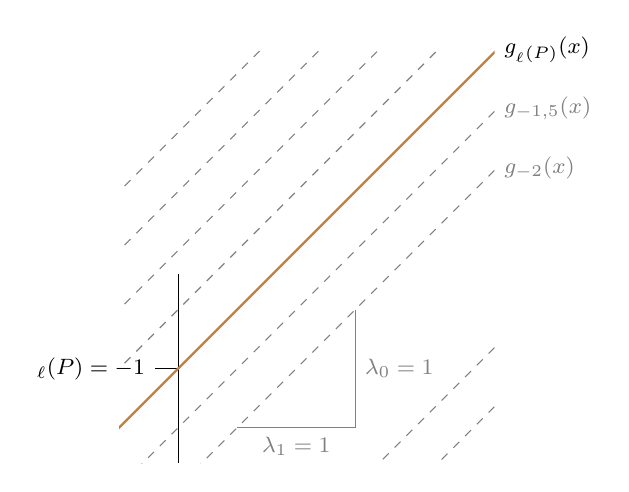
\begin{tikzpicture}[scale=1.5,descr/.style={fill=white,inner sep=2.5pt}]
      \def\myPoints{0/0,2/1}
      \def\myPath{ -- (2,1)}
      \myPlotFunction[nogrid]{\myPoints}{\myPath}{2}{0}{1}{}


      \draw (0,-.2) -- (0,-1.8);
      \draw (0,-1) -- (-.2,-1);
      \node[left] at (-.2,-1) {\footnotesize$\ord_\ell(P)=-1$};
      \node[right] at (2.68,1.7) {\footnotesize$g_{\ord_\ell(P)}(x)$};
      \node[right,gray] at (2.68,1.2) {\footnotesize$g_{-1,5}(x)$};
      \node[right,gray] at (2.68,0.7) {\footnotesize$g_{-2}(x)$};

      \clip (-0.5,-1.8) rectangle (2.68,1.7);
      %\draw[gray] (0,-2) -- ++(225:-1cm) -- ++(45:2.3cm);
      \draw[gray,dashed] (0,-4) ++(225:5cm) -- ++(45:8.8cm);
      \draw[gray,dashed] (0,-3.5) ++(225:5cm) -- ++(45:8.8cm);
      %\draw[gray,dashed] (0,-3) ++(225:5cm) -- ++(45:8.8cm);
      %\draw[gray,dashed] (0,-2.5) ++(225:5cm) -- ++(45:8.8cm);
      \draw[gray] (.5,-1.5) -- node[below]{\footnotesize$\lambda_1=1$} (1.5,-1.5) 
        -- node[right]{\footnotesize$\lambda_0=1$} (1.5,-.5);
      \draw[gray,dashed] (0,-2) ++(225:5cm) -- ++(45:8.8cm);
      \draw[gray,dashed] (0,-1.5) ++(225:5cm) -- ++(45:8.8cm);
      \draw[gray,dashed] (0,-0.5) ++(225:5cm) -- ++(45:8.8cm);
      \draw[gray,dashed] (0,0) ++(225:5cm) -- ++(45:8.8cm);
      \draw[gray,dashed] (0,0.5) ++(225:5cm) -- ++(45:8.8cm);
      \draw[gray,dashed] (0,1) ++(225:5cm) -- ++(45:8.8cm);
      \draw[brown,thick] (0,-1) ++(225:5cm) -- ++(45:8.8cm);
      \end{tikzpicture}
    \end{center}
  \caption{Zu Bemerkung \ref{bem:bildlichlNorm}.}
  \label{fig:bildlichlNorm}
\end{figure}
\end{bem}
\begin{bem}
Nach \cite[Seite 25]{sabbah_cimpa90} gilt, dass man
$\ord_\ell(PQ)=\ord_\ell(P)+\ord_\ell(Q)$ hat und falls $\lambda_0\neq 0$, hat
man auch, das $\ord_\ell([P,Q])\leq \ord_\ell(P)+\ord_\ell(Q)-1$.
\end{bem}

Nun können wir die aufsteigende Filtration $\,^\ell V\cD_{\hat K}$, welche mit
$\Z$ indiziert ist, durch
\[
\,^\ell V_\lambda\cD_{\hat K}:=\{P\in\cD_{\hat K}\mid \ord_\ell(P)\leq \lambda\}
\]
definieren.
Falls $\lambda_0\neq 0$, ist der gradierte Ring $gr^{\,^\ell V}\cD_{\hat
K}\bydef \bigoplus_{\lambda \in \Z}gr_\lambda^{\,^\ell V}\cD_{\hat K}$ ein
kommutativer Ring. Bezeichne die Klasse von $\partial_x$ in dem Ring durch
$\xi$, dann ist der Ring isomorph zu $\hat K[\xi]$.
\begin{defn}[$\ell$-Symbol]
Sei $P\in \cD_{\hat K}$, so ist $\sigma_\ell(P)$ definiert als die Klasse von
$P$ in $gr_{\ord_\ell(P)}^{\,^\ell V}\cD_{\hat K}$ und wird als das
\emph{$\ell$-Symbol} bezeichnet.
\end{defn}
\begin{bsp} \label{exmp:lSymbol}
Zum Beispiel ist $\sigma_\ell(x^a\partial_x^b)=x^a\xi^b$ für alle
$a\in\Z$, $b\in\N$. Ein komplexeres Beispiel ist $P=x^2\partial_x+1$. Betrachte
dazu ein $\ell(s_0,s_1)=\lambda_0s_0+\lambda_1s_1$ mit $\lambda_0\neq0$ und
unterscheide die folgenden drei Fälle:
\begin{itemize}
\item $\lambda_0-\lambda_1>0$, so ist $\sigma_\ell=x^2\xi$.
\item $\lambda_0=\lambda_1$, so ist $\sigma_\ell=x^2\xi+1$.
\item $\lambda_0-\lambda_1<0$, so ist $\sigma_\ell=1$.
\end{itemize}
In Abbildung \ref{fig:lSymbol} sind, für jeden der Fälle, jeweils das
Newton-Polygon, zusammen mit
$g_{\ord_\ell(P)}(x)=\frac{\lambda_0}{\lambda_1}+\ord_\ell(P)$ in Braun,
eingezeichnet. Das $\ell$-Symbol von $P$ sind, bildlich vorgestellt, jeweils
die Monome, die auf $g_{\ord_\ell(P)}(x)$ \glqq liegen\grqq. Mit dieser
Vorstellung ist es klar, dass $\sigma_\ell(P)$ genau dann aus mehr als einem
Monom besteht, wenn $\Lambda:=\frac{\lambda_0}{\lambda_1}$ ein Slope von $P$
ist.
\begin{figure}[H] % htbp
  \begin{minipage}[hbt]{0,32\textwidth}
    \begin{center}
      \begin{tikzpicture}[scale=1.5,descr/.style={fill=white,inner sep=2.5pt}]
      \def\myPoints{0/0,1/1}
      \def\myPath{ -- node[descr]{$1$} (1,1)}
      \myPlotFunction{\myPoints}{\myPath}{1}{0}{1}{}
      \draw[brown,thick] (1,1) -- ++(60:.5cm)
        node[right]{\footnotesize$\lambda_0-\lambda_1>0$};
      \draw[brown,thick] (1,1) -- ++(240:1.5cm);  
      \end{tikzpicture}
    \end{center}
  \end{minipage}
  \begin{minipage}[hbt]{0,32\textwidth}
    \begin{center}
      \begin{tikzpicture}[scale=1.5,descr/.style={fill=white,inner sep=2.5pt}]
      \def\myPoints{0/0,1/1}
      \def\myPath{ -- (1,1)}
      \myPlotFunction{\myPoints}{\myPath}{1}{0}{1}{}
      \draw[brown,thick] (1,1) -- ++(45:.5cm)
        node[right]{\footnotesize$\lambda_0=\lambda_1$};
      \draw[brown,thick] (1,1) -- ++(225:1.8cm);  
      \end{tikzpicture}
    \end{center}
  \end{minipage}
  \begin{minipage}[hbt]{0,32\textwidth}
    \begin{center}
      \begin{tikzpicture}[scale=1.5,descr/.style={fill=white,inner sep=2.5pt}]
      \def\myPoints{0/0,1/1}
      \def\myPath{ -- node[descr]{$1$} (1,1)}
      \myPlotFunction{\myPoints}{\myPath}{1}{0}{1}{}
      \draw[brown,thick] (0,0) -- ++(30:1.5cm)
        node[right]{\footnotesize$\lambda_0-\lambda_1<0$};
      \draw[brown,thick] (0,0) -- ++(210:.5cm);  
      \end{tikzpicture}
    \end{center}
  \end{minipage}
  \caption{Zu Beispiel \ref{exmp:lSymbol}.}
  \label{fig:lSymbol}
\end{figure}
\end{bsp}
\begin{bem}
Ist $P\in \cD_{\hat K}$ geschrieben als
$P=\sum_i\sum_j\alpha_{ij}x^j\partial_x^i$.
So erhält man $\sigma_\ell(P)$ durch die Setzung
\[
\sigma_\ell(P)=\sum_{\{(i,j)\mid\ell(i,i-j)=\ord_\ell(P)\}}\alpha_{ij}x^j\xi^i \,.
\]
\end{bem}
\begin{comment}
\begin{proof}
TODO
\end{proof}
\end{comment}

\begin{bem}
Bei \cite{sabbah_cimpa90} wird der Buchstabe $L$ anstatt $\ell$ für
Linearformen verwendet, dieser ist hier aber bereits für $\Ckt$ reserviert.
Dementsprechend ist die Filtrierung dort als $\,^L V\cD_{\hat K}$ und das
$\ell$-Symbol als $L$-Symbol zu finden.
\end{bem}
\begin{bem}[Stützfunktion]
Die Funktion
\[
\omega_P:[0,\infty)\rightarrow\R, \omega_P(t):=\inf\{v-tu \mid (u.v) \in N(P)\}
\]
heißt Stützfunktion und wird in \cite{ZulaBarbara} als Alternative zur hier
definierten Filtrierung verwendet.
Wenn $\ell(x_0,s_1)$ wie oben aus $\Lambda$ entstanden ist, so gilt
\[
\omega_P(\Lambda)=ord_\ell(P) \,.
\]
\end{bem}

\section{Levelt-\!Turrittin-\!Theorem}
\begin{comment}
Das Levelt-Turrittin-Theorem ist ein Satz, der hilft, meromorphe Zusammenhänge
in ihre irreduziblen Komponenten zu zerlegen.
\end{comment}

\begin{thm}[Levelt-\!Turrittin-\!Theorem]
\label{thm:LT}
Sei $\cM_{\hat K}$ ein formaler meromorpher Zusammenhang, so gibt es eine
ganze Zahl $p$, so dass der Zusammenhang $\rho^+\cM_{\hat K}$, mit
$\rho:t\mapsto x:=t^p$, isomorph zu einer direkten Summe von formalen
elementaren meromorphen Zusammenhänge ist.
\begin{comment}
\cite[Thm 5.4.7]{sabbah_cimpa90}
\end{comment}
\end{thm}
\begin{bem}
Man kann auch allgemeiner für $\rho$ ein beliebiges Polynom, vom grad $p$
nehmen.
\end{bem}
\begin{comment}
Der folgende Beweis stammt hauptsächlich aus \cite[Seite 35]{sabbah_cimpa90}.
\end{comment}
\begin{proof}[Beweisskizze]
Zum Beweis wird Induktion auf die lexicographisch geordnetem Paare
$(\dim_{\hat K}\cM_{\hat K},\kappa)$ angewendet. Wobei
$\kappa\in\N\cup\{\infty\}$ dem größtem Slope von $\cM_{\hat K}$, falls dieser
ganzzahlig ist, entspricht. Sonsts wird $\kappa=\infty$ gesetzt. In jedem
Induktionsschritt wird entweder die Dimension oder das $\kappa$ verringert.

\begin{comment}
TODO: Induktionsanfang und -schritt kennzeichnen
\end{comment}
Wir nehmen oBdA an, dass $\cM_{\hat K}$ genau einen Slope $\Lambda$ hat, sonst
Teile $\cM_{\hat K}$ mittels Satz \ref{thm:Split-after-slopes} in meromorphe
Zusammenhänge mit je einem Slope und wende jeweils die Induktion an.
Mit $\Lambda=:\frac{\lambda_0}{\lambda_1}$ (vollständig gekürtzt) definieren
wir die dem Slope entsprechende Linearform
$\ell(s_0,s_1):=\lambda_0s_0+\lambda_1s_1$.  
Wir nehmen oBdA auch an, dass $\ord_\ell(P)=0$. Dies geht nach Bemerkung
\ref{bem:NPverschieben}.
Da $\ell$ zu einem Slope von
$P$ gehört, besteht $\sigma_\ell(P)$ aus zumindest zwei Monomen.
Schreibe
\begin{align*}
\sigma_\ell(P)&=\sum_{\ell(i,i-j)=\ord_\ell(P)}\alpha_{ij}x^j\xi^i\\
  &=\sum_{\ell(i,i-j)=0}\alpha_{ij}x^j\xi^i
\end{align*}
und setze $\theta:=x^{\lambda_0+\lambda_1}xi^{\lambda_1}$ so erhalten wir
\[
\sigma_\ell(P) = \sum_{k\geq 0}\alpha_k\theta^k \,,
\]
wobei $\alpha_0\neq0$ ist.

\paragraph{Erster Fall: $\lambda_1=1$.} Das bedeutet, dass der Slope ganzzahlig
ist. Betrachte die Faktorisierung
\[
\sigma_\ell(P)=
  \epsilon\prod_{\beta\text{ Nullstelle}}(\theta-\beta)^{\gamma_\beta}\,.
\]
Wobei $\epsilon\in\C^\times$ eine Konstante ist.  Sei $\beta$  eine der
Nullstellen, so setze $\psi(x):=(\beta_0/\lambda_0)x^{-\lambda_0}$ und
betrachte $\cM_{\hat K}\otimes_{\hat K} \sE_{\hat K}^{\psi}$.
Sei $P$ ein Minimalpolynom von $\cM_{\hat K}$, dann ist nach Lemma
\ref{lem:twistRechenregel} ein Minimalpolynom von 
$\cM_{\hat K}\otimes_{\hat K} \sE_{\hat K}^{\psi}$ gegeben durch
\begin{align*}
P'(x,\partial_x)&=P(x,\partial_x-\frac{\partial \psi}{\partial x})
\\&=P(x,\partial_x+\frac{\beta}{x^{\lambda_0+1}})
\end{align*}
mit Koeffizienten in
$\Cfx$.
Des weiteren ist $\sigma_\ell(P')=\sum_{k\geq 0}\alpha_k(\theta+\beta_0)^k$.
Wir unterscheiden nun 2 Unterfälle:
\begin{enumerate}
\item \textbf{Die Determinanten Gleichung $\sigma_\ell(P)$ hat nur eine
Nullstelle.}
In diesem fall wurde die maximale Steigung echt verringert.
\begin{comment}TODO: Hier weiter \end{comment}
\item \textbf{Die Determinanten Gleichung $\sigma_\ell(P)$ hat mehrere
Nullstellen.}
In diesem fall hat $\cM_{\hat K}\otimes_{\hat K} \sE_{\hat K}^{\psi}$ mehr als
einen Slope und kann deshalb mit Satz \ref{thm:Split-after-slopes} in eine
direkte Summe von Meromorphen Zusammenhängen, mit echt niedrigerer Dimension,
zerlegt werden.
\begin{comment}TODO: Hier weiter \end{comment}
\end{enumerate}
In beiden Unterfällen muss danach das Twisten, nach Anwenden der Induktion,
durch ein tensorieren mit $\sE_{\hat K}^{-\psi}$ rückgängig gemacht werden.

\paragraph{Zweiter Fall: $\lambda_1\neq1$ (bzw. $\kappa = +\infty$).} 
In diesem Fall ist einzige Slope $\Lambda$ nicht ganzzahlig. Mache deshalb
einen pull-back mit $\lambda_1$. Sei $\rho:t\mapsto x:=t^{\lambda_1}$ und
erhalte $P'$ so dass $\rho^*\cM_{\hat K}=\cD_{\hat L}/\cD_{\hat L}\cdot P'$.
Nach Lemma \ref{lem:slope-pb-multiplikation} hat $P'$ den einen Slope
$\Lambda'=\Lambda\cdot\lambda_1=\lambda_0\in\N$.
\begin{comment}
Damit können wir nun die zugehörige Linearform $\ell':=\lambda_0s_0+s_1$
definieren. Es gilt dass
\[
\sigma_{\ell'}(P')=\dots
\]
ist, welches zumindest zwei unterschiedliche Nullstellen hat. Nun wendet man
den zweiten Unterfall des ersten Fall an.
\end{comment}
\end{proof} % ende von beweis zu levelt aus sabbah_cimpa90
\begin{bem}
Das Levelt-Turrittin-Theorem ist auch in \cite[Thm 5.4.7]{sabbah_cimpa90}, aber
ohne ausführlichen Beweis, zu finden.
Eine sehr detailierte Version dieses Beweises, ist beispielsweise in \cite[Thm
5.16]{DiplHedwig} ausformuliert.
\end{bem}

\begin{comment}
\subsection{Sabbah's Refined version}
\begin{prop}
\cite[Prop 3.1]{sabbah_Fourier-local}
Jeder irreduzible endlich dimensionale formale meromorphe Zusammenhang
$\cM_{\hat L}$ ist isomorph zu $\rho_+(\sE^\phi\otimes_{\hat K} S)$, wobei
$\phi\in x^{-1}\C[x^-1]$, $\rho:x\mapsto t=x^p$ mit grad $p\geq1$ minimal bzgl.
$\phi$ (siehe \cite[Rem 2.8]{sabbah_Fourier-local}), und $S$ ist ein Rang $1$
$\hat K$-Vektor Raum mit regulärem Zusammenhang.
\end{prop}
\begin{proof}
\cite[Prop 3.1]{sabbah_Fourier-local}
\end{proof}

\begin{thm}[Refined Turrittin-Levelt]
\cite[Cor 3.3]{sabbah_Fourier-local}
Jeder endlich dimensionale meromorphe Zusammenhang $\cM_{\hat K}$ kann in
eindutiger weiße geschrieben werden als direkte Summe $\bigoplus
El(\rho,\phi,R)\bydef\bigoplus\rho_+(\sE^\phi)\otimes R$, so dass
jedes $\rho_+\sE^\phi$ irreduzibel ist und keine zwei $\rho_+\sE^\phi$ isomorph
sind.
\end{thm}
\begin{proof}
\cite[Cor 3.3]{sabbah_Fourier-local}
\end{proof}
\end{comment}

% vim: set ft=tex :
